\documentclass[11pt,a4paper]{article}

\usepackage[english]{babel}
\usepackage[T1]{fontenc}
%\usepackage[latin1]{inputenc}

\usepackage{amsmath}
\usepackage{multirow}
%\usepackage[margin=2cm]{geometry}
\usepackage[dvipsnames]{xcolor}

\usepackage{graphicx}
\usepackage{amssymb}
\usepackage{mathrsfs}
\usepackage{subcaption}
\usepackage{setspace} 

\definecolor{AB}{rgb}{0,0.3961,0.7412}

\usepackage[bookmarksnumbered=true]{hyperref} 
\hypersetup{
     colorlinks = true,
     linkcolor = AB,
     anchorcolor = AB,
     citecolor = AB,
     filecolor = AB,
     urlcolor = AB
 }
\usepackage{enumitem}
\allowdisplaybreaks

\addtolength{\oddsidemargin}{-.8in}
\addtolength{\evensidemargin}{-.65in}
\addtolength{\textwidth}{1.68in}
\addtolength{\topmargin}{-.875in}
\addtolength{\textheight}{1.15in}

\usepackage{titlesec}
\titleformat{\section}{\fontsize{12}{14}\sc}{\thesection}{1em}{}[]
\titleformat{\subsection}{\fontsize{11}{12}\sc}{\thesubsection}{1em}{}[]
\titleformat{\subsubsection}{\fontsize{10}{11}\sc}{\thesubsection}{1em}{}[]
 
 \setlength{\parindent}{0pt}
 
\usepackage{tocloft}
\renewcommand{\cfttoctitlefont}{\sc}
\renewcommand{\cftsecfont}{\sc}
\renewcommand{\cftsubsecfont}{\sc}

\usepackage{abstract}
\renewcommand\abstractnamefont{\sc}

\usepackage[round]{natbib}

 
\begin{document}
\thispagestyle{empty}

\begin{flushleft} 
\includegraphics[width=1.0\textwidth]{headers}   \end{flushleft}

\vskip0.5cm
\begin{spacing}{2} {\Large\sc\noindent Exercise List 1}
\end{spacing}

\vfill

\begin{spacing}{1.2}
{\large\sc  Antonio Felype Ferreira Maciel - 576261}\\

{\noindent \large \sc Master's Course in Teleinformatics Engineering}\\
{\noindent \large \sc Federal University of Ceará}\\

{\noindent \large \sc TIP8300 - Nonlinear System Optimization}
\end{spacing}

\newpage 

% \tableofcontents

\newpage

%\begin{abstract}
% This report provides a concise introduction to Up-flow Anaerobic Sludge Blanket reactor, outlines its applications in Brazil, and explains the model we are using for simulations. We discuss our intentions for using this model, the challenges we are currently facing and our next steps. 
%\end{abstract}

\section*{Chapter 2 -- Convex Sets}

\begin{itemize}
    \item[\textbf{2.11}] Define the square $S = \{x \in \mathbf{R}^2 \,\vert\, 0 \leq x_i \leq 1, \, i = 1, 2\}$, and the disk $D = \{x \in \mathbf{R}^2 \, \vert \, \|x\|_2 \leq 1\}$. Are the following statements true or false?
    \item[] \begin{itemize}
        \item[(a)] $S \cap D$ is convex.
            
        A set is convex if, for every pair of points $x$ and $y \in C$ and every $\lambda \in [0, 1]$, the point $z = \lambda x + (1-\lambda)y$ also belongs to C. 

        \begin{equation*}
            S = \{(x_1, x_2) \vert 0 \leq x_1 \leq 1, 0 \leq x_2 \leq 1\}
        \end{equation*}
        
        For $x = (x_1, x_2)$ and $y = (y_1, y_2) \in S$ and $\lambda \in [0, 1]$, $z = \lambda x + (1- \lambda)y$, which means that:
        
        \begin{equation*}
            \begin{aligned}
                z_1 = & \lambda x_1 + (1- \lambda)y_1\\ 
                z_2 = & \lambda x_2 + (1- \lambda)y_2.
            \end{aligned}
        \end{equation*}

        Since $x_1$ and $x_2$ vary between 0 and 1, for every of these extremities and for the values of $\lambda$, $z_1$ and $z_2$ also belong to $S$. This way, $S$ is convex.

        \begin{equation*}
            D = \{x \in \mathbf{R}^2 \,\vert\, \Vert x \Vert_2\}
        \end{equation*}

        For $D$ to be convex, for any two points $x_1$, $x_2 \in D$ and for any $\lambda \in [0,1]$, the combination

        \begin{equation*}
            z = x_1 \lambda + (1-\lambda)x_2
        \end{equation*}

        must belong to $D$. Therefore $\Vert z \Vert_2 \leq 1$ must be true.

        Using the triangle inequality

        \begin{equation*}
            \begin{aligned}
                \Vert z \Vert_2 \leq & \, \Vert x_1 \Vert_2 \lambda + (1 - \lambda)\Vert x_2 \Vert_2\\
                \Vert x_1\lambda + (1-\lambda)\Vert_2 \leq & \, \Vert x_1 \Vert_2 \lambda + (1-\lambda) \Vert x_2\Vert_2.
            \end{aligned}
        \end{equation*}

        Since $x_1, x_2 \in D$, $\Vert x_1 \Vert_2 \leq 1$ and $\Vert x_2 \Vert_2 \leq 1$. Then, for $x_1 = x_2 = 1$

        \begin{equation*}
            \begin{aligned}
                \Vert z \Vert_2 \leq \, & \lambda(1-\lambda) = 1\\
                \Vert z \Vert_2 \leq \, & 1.
            \end{aligned}
        \end{equation*}

        This way, $D$ is also convex. Since both sets are convex and intersection preserves convexity, the sentence is \textbf{true}. $S$, in orange, and $D$ in blue are shown in Figure~\ref{fig:SD}. Their intersection is shown in Figure~\ref{fig:intersection}.
 
        \item[(b)] $S \cup D$ is convex.
        
        Union does not necessarily preserve convexity. But from Figure~\ref{fig:union}, it is possible to see a line between every two points in the union in the set. Therefore, the sentence is \textbf{true}.

        \item[(c)] $S \setminus D$ is convex.  
        
        The set generated by the difference operation is shown in Figure~\ref{fig:difference}. It is possible to see that not all lines between two points in the set belong to $S \setminus D$. Therefore, the sentence is \textbf{false}.

        
        \begin{figure}[!htb]
            \centering
            \begin{subfigure}[b]{0.24\textwidth}
                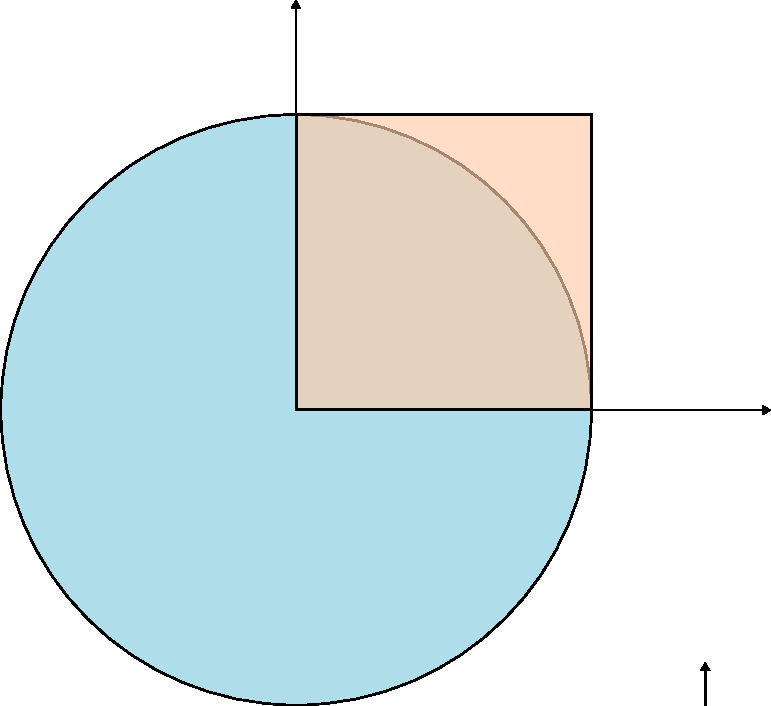
\includegraphics[width=\textwidth]{figures/SD.pdf}
                \caption{}\label{fig:SD}
            \end{subfigure}
            \begin{subfigure}[b]{0.24\textwidth}
                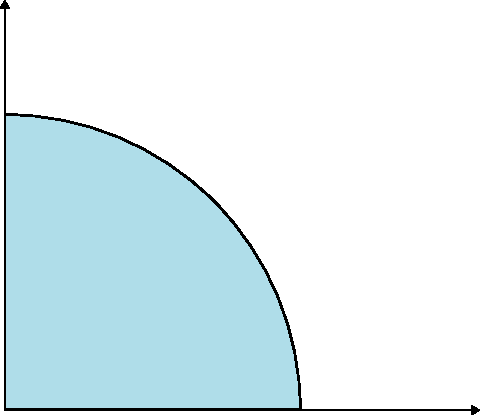
\includegraphics[width=\textwidth]{figures/intersection.pdf}
                \caption{}\label{fig:intersection}
            \end{subfigure}
            \begin{subfigure}[b]{0.24\textwidth}
                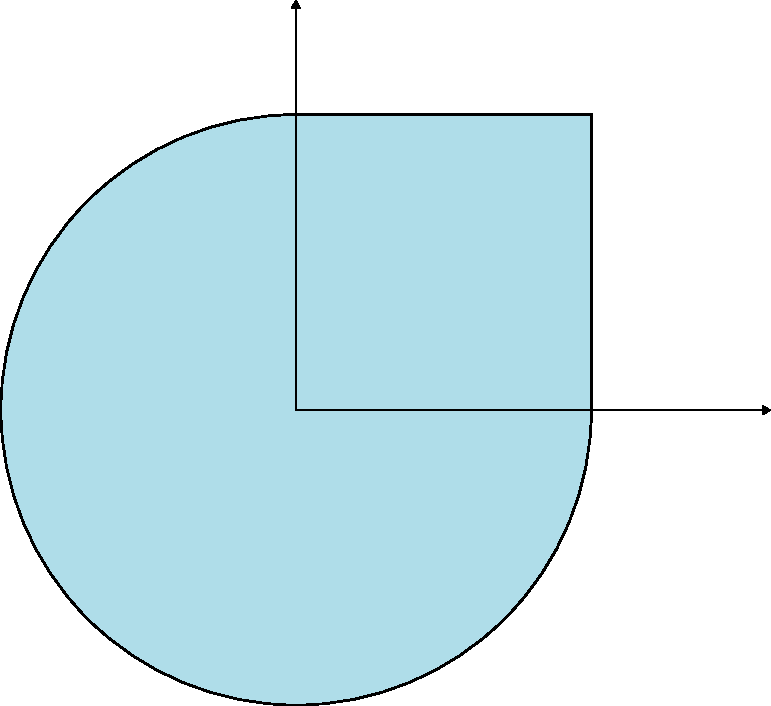
\includegraphics[width=\textwidth]{figures/SUD.pdf}
                \caption{}\label{fig:union}
            \end{subfigure}
            \begin{subfigure}[b]{0.24\textwidth}
                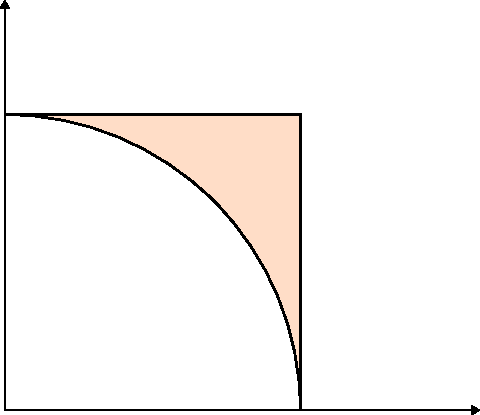
\includegraphics[width=\textwidth]{figures/difference.pdf}
                \caption{}\label{fig:difference}
            \end{subfigure}
        \end{figure}
    \end{itemize}

    \begin{figure}[!htb]
        \centering
        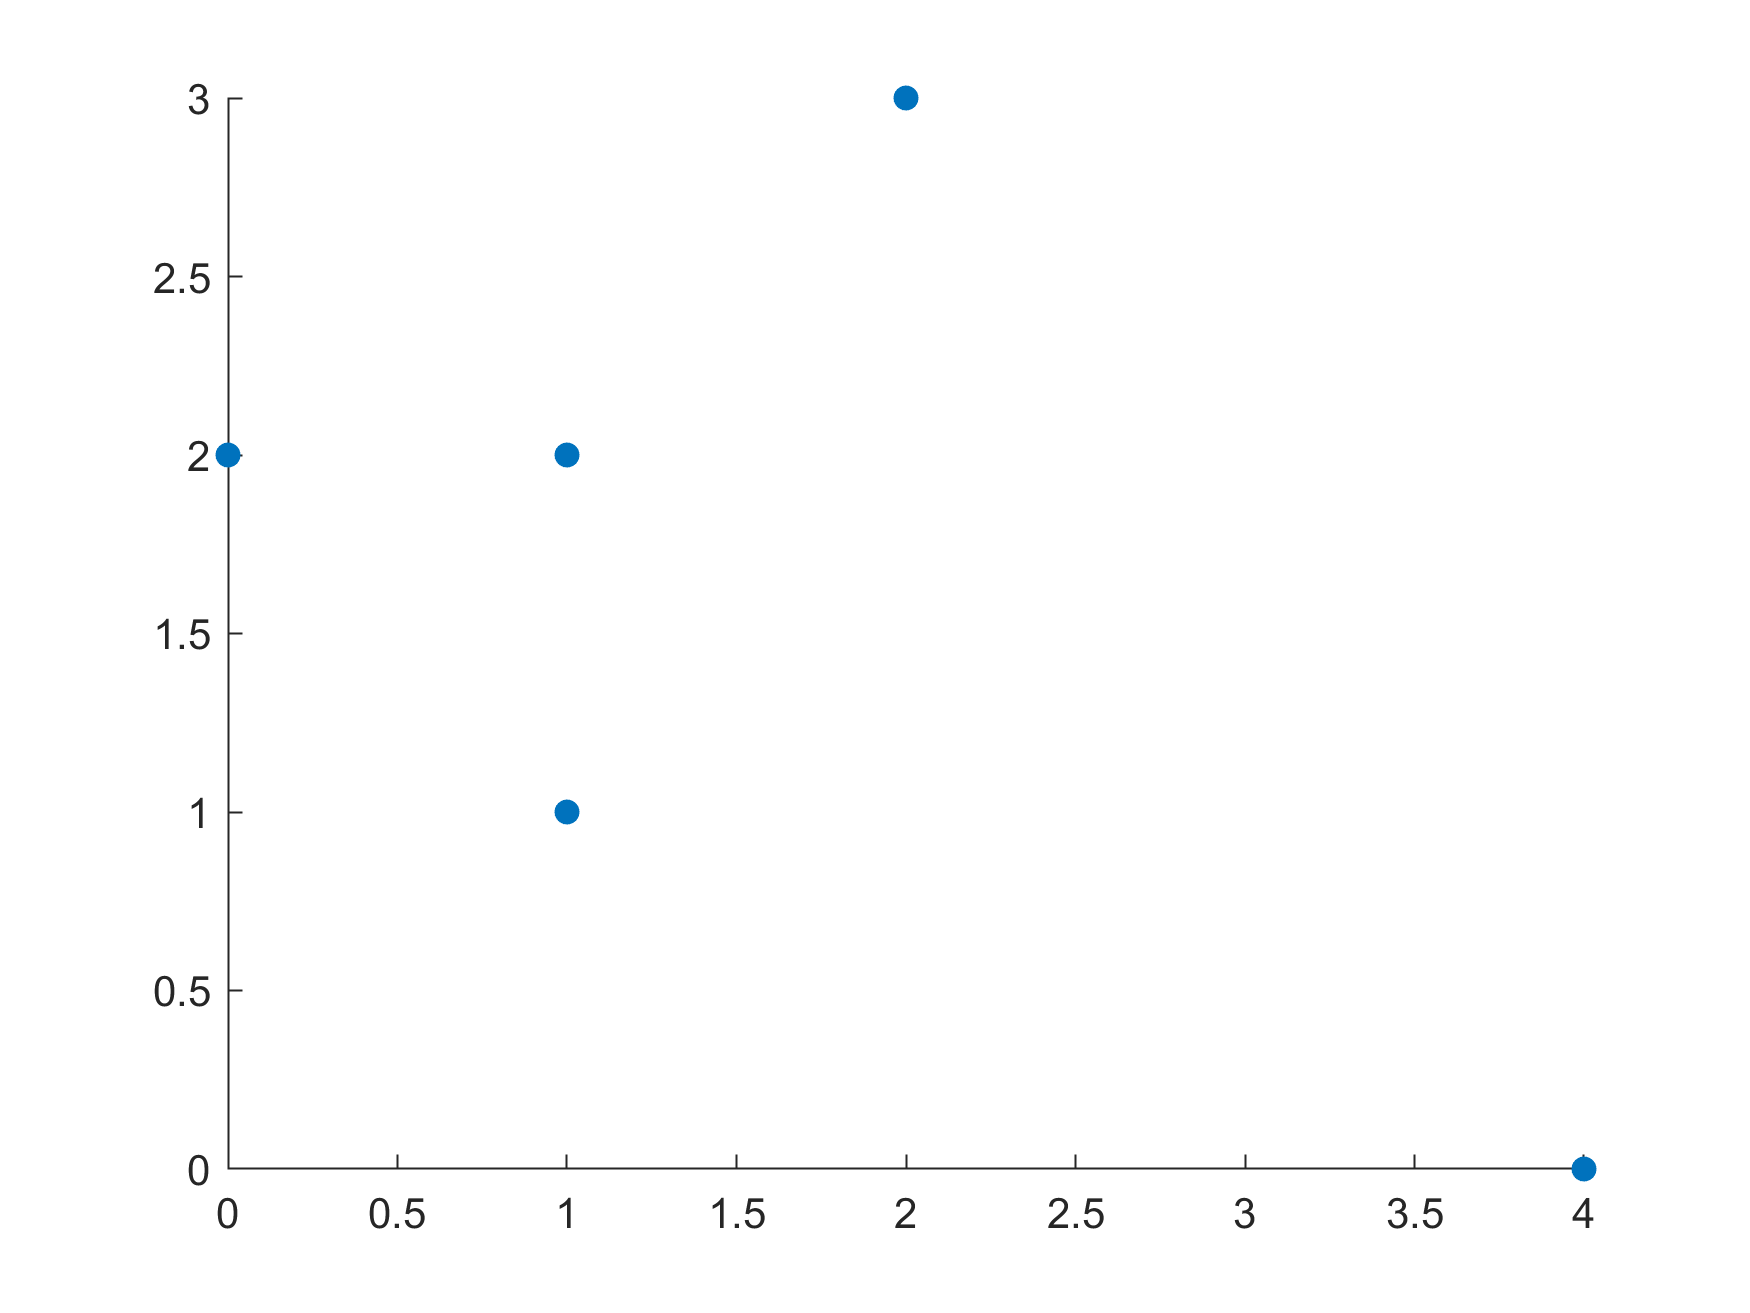
\includegraphics[width=0.5\textwidth]{figures/question2.png}
        \caption{Elements of set $S$.}\label{fig:question2}
    \end{figure}

    \item[\textbf{2.13}] \textit{Minimal and minimum elements}. Consider the set $S = \{(0,2), (1,1), (2,3), (1,2), (4,0)\}$ (Figure~\ref{fig:question2}). Are the following statements true or false?

    \item[] \begin{itemize}
        \item[(a)] (0,2) is the minimum element of $S$.
        
        \textbf{False}, since $(0,2)$ is not comparable to $(1,1)$ and to $(4,0)$.

        \item[(b)] (0,2) is a minimal element of $S$.
        
        \textbf{True}, since no element is smaller than $(0,2)$.

        \item[(c)] (2,3) is a minimal element of $S$.
        
        \textbf{False}, the element $(0,2)$ is strictly smaller than $(2,3)$.

        \item[(d)] (1,1) is a minimal element of $S$.
        
        \textbf{True}, since no element is smaller than $(1,1)$.
    \end{itemize}
        Here, minimum and minimal are with respect to the nonnegative orthant $K = \mathbf{R}_+^2$.
    \item[\textbf{2.16}] \textit{Generalized inequality}. Let $K = \{(x_1,x_2) \, \vert \, 0 \leq x_1 \leq x_2\}$. Are the following statements true or false?
    \item[] \begin{itemize}
        \item[(a)] $(1,3) \preceq_K (3,4)$.
        
        \textbf{True}, since $1 \leq 3$ and $3 \leq 4$.

        \item[(b)] $(-1,2) \in K^*$.
        
        $K^*$ is the dual cone of $K$:
        \begin{equation*}
            K^* = \{y \,\vert\, x^T y \geq 0 \,\forall\, x \in K\}
        \end{equation*}

        \begin{equation*}
            \begin{aligned}
                x = & (x_1, x_2) \text{ and } y = (y_1, y_2) \\
                x^T y = & \begin{bmatrix}
                    x_1 \\
                    x_2
                \end{bmatrix}
                \begin{bmatrix}
                    y_1 & y_2
                \end{bmatrix}\\
                x^T y = & x_1y_1 + x_2 y_2 \geq 0 \\
                = & x_1 \cdot (-1) + x_2 \cdot 2 \geq 0\\
                = & -x_1 + 2x_2
            \end{aligned}
        \end{equation*}

        For the sentence to be true, $2x_2 \geq x_1$ must be valid for all $x \in K$, and it is. This way, $(-1, 2) \in K^*$ and the sentence is \textbf{true}.

        \item[(c)] The unit circle (\textit{i.e.}, $\{x \, \vert \, \|x\|_2 = 1\}$) does not contain a minimum element with respect to $K$.
        
        It is \textbf{true}. The unit circle has elements in all quadrants, while $K$ is defined only in the first quadrant. In this way, there are elements that cannot be compared, which is required for an element to be minimum.

        \item[(d)] The unit circle does not contain a minimal element with respect to $K$.
        
        The sentence is \textbf{false}. With respect to the relation $K$, only the points in the first quadrant of the unit circle are considered. The blue area in Figure~\ref{fig:circle-216} contains the points that obey $K$. The points that satisfy both $K$ and the definition of the unit circle are those on the arc above this blue area. When we consider the points on the arc, it becomes evident that no point dominates another, and therefore, there is no point greater than another on the arc. Because of this, all the points on the arc are minimal.

        \begin{figure}[!htb]
            \centering
            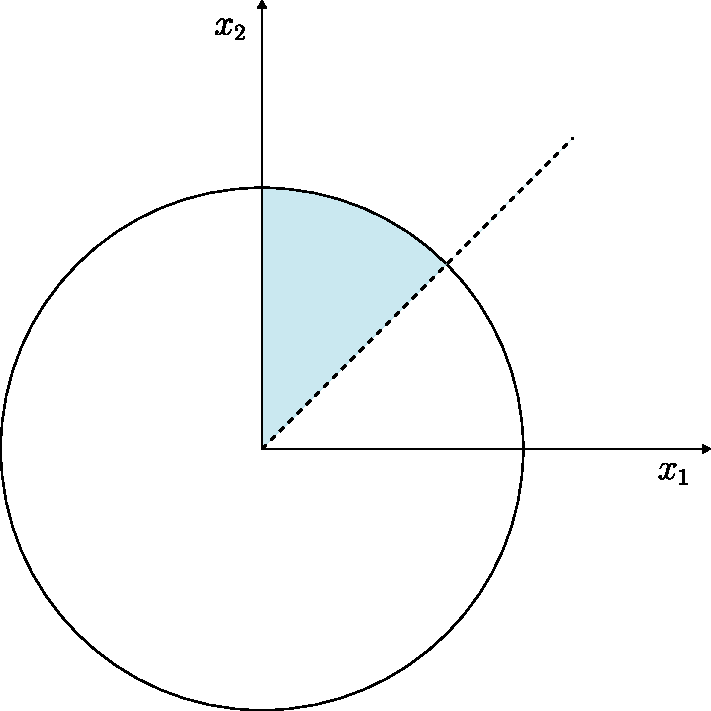
\includegraphics[width=0.5\textwidth]{figures/circle216.pdf}
            \caption{Unit circle for question 2.16.}\label{fig:circle-216}
        \end{figure}
        
    \end{itemize}
\end{itemize}

\section*{Chapter 3 -- Convex Functions}

\begin{itemize}
    \item[\textbf{3.33}] \textit{DCP rules}. The function $f(x,y) = \sqrt{1 + x^4/y}$, with $\textbf{dom} f = \mathbf{R}\times\mathbf{R}_{++}$, is convex. Use disciplined convex programming (DCP) to express $f$ so that it is DCP convex. You can use any of the following atoms
    \item[]\begin{itemize}
        \item[] \texttt{inv\_pos(u)}, which is $1/u$, with domain $\mathbf{R}_{++}$
        \item[] \texttt{square(u)}
        \item[] \texttt{sqrt(u)}
        \item[] \texttt{geo\_mean(u,v)}
        \item[] \texttt{quad\_over\_lin(u,v)}
        \item[] \texttt{norm2(u,v)}
    \end{itemize}

    You may also use addition, subtraction, scalar multiplication, and any constant functions. Assume that DCP is sign-sensitive, \textit{e.g.}, \texttt{square(u)} is known to be increasing in $u$ for $u \geq 0$.

    \texttt{$\sqrt{y}$ =  cp.sqrt(y)}

    \texttt{$\cfrac{x^2}{\sqrt{y}}$  =  cp.quad\_over\_lin($x$,$\sqrt{y}$)}

    \texttt{$\sqrt{1 + \cfrac{x^4}{y}}$ = cp.norm2(1, $\cfrac{x^2}{\sqrt{y}}$)} 

    \texttt{f  = cp.norm2(1, cp.quad\_over\_lin(x,cp.sqrt(y)))}

    \item[\textbf{3.38}] \textit{Curvature of some functions}. Determine the curvature of the functions below. Your responses can be: affine, convex, concave, and none (meaning, neither convex nor concave).
    \item[] \begin{itemize}
        \item[(a)] $f(x) = \min\{2,x,\sqrt{x}\}$, with $\textbf{dom}\, f = \mathbf{R}_+$
        
        Since $f(x)$ is a piecewise function, we can analyse each of its components. Firstly, $2$ is constant. Therefore, it is both convex and concave. Then $x$ is linear, which is also convex and concave. Finally, $\sqrt{x}$ is concave for $x \geq 0$ since its second-order derivative is nonnegative for its domain. This function can be thought as a piecewise function

        \begin{equation*}
            f(x) = \begin{cases}
                x & 0 \leq x \leq 1\\
                \sqrt{x} & 1 < x < 2\\
                2 & x \geq 2
            \end{cases}
        \end{equation*}

        \noindent where its parts can be thought as concave functions. Since the minimum operation preserves concavity, $f(x)$ is concave. When checking the curvature of $f(x)$ using \texttt{cvxpy}, the result is that the curvature is concave. 

        \item[(b)] $f(x) = x^3$, with $\textbf{dom} \, f = \mathbf{R}$
        
        Following the second-order condition, a function is convex if $f''(x) \geq 0$ for all $x$ in the domain. The second derivative of $x^3$ is $6x$. Since the domain is the whole real set $\mathbf{R}$, the condition is not attended. Then $f(x)$ is not convex. For a function to be concave, its second-order derivative must be less or equal to zero for all its domain. This is not true for $f(x)$, so the curve is not convex nor concave. 

        \item[(c)] $f(x) = x^3$, with $\textbf{dom} \, f = \mathbf{R}_{++}$
        
        For the specified domain, the function attends the second-order condition. Therefore, $f(x)$ is convex. 

        \item[(d)] $f(x,y) = \sqrt{x \min\{y,2\}}$, with $\mathbf{dom} \, f = \mathbf{R}_+^2$
        
        We can think of $f(x,y)$ as

        \begin{equation*}
            f(x,y) = \begin{cases}
                \sqrt{xy} & 0 \leq y \leq 2\\
                \sqrt{2x} & y > 2
            \end{cases}.
        \end{equation*}

        For the first interval, $0 \leq y \leq 2$, $f(x,y) = \sqrt{xy}$. The Hessian of $f(x,y)$ is

        \begin{equation*}
            \begin{bmatrix}
                    -\cfrac{y^2}{4 \sqrt{(x y)^3}} & \cfrac{1}{2 \sqrt{x y}} - \cfrac{x y}{4 \sqrt{(x y)^3}} \\
                    \cfrac{1}{2 \sqrt{x y}} - \cfrac{x y}{4 \sqrt{(x y)^3}} & -\cfrac{x^2}{4 \sqrt{(x y)^3}}
            \end{bmatrix}.
        \end{equation*}

        The eigenvalues of the Hessian are $0$ and $-\cfrac{x^2 + y^2}{4\sqrt{(xy)^3}}$. Since the eigenvalues are non-positive, the Hessian is negative semidefinite, and the function is concave. 

        For the second interval, $y > 2$, $f(x, y) = \sqrt{2x}$. The second-order derivative of $f(x,y)$ is $-\cfrac{\sqrt{2}}{4\sqrt{x^3}}$, which is negative for the whole interval. Therefore, $f(x,y) = \sqrt{2x}$ is concave. 

        Since both parts of the function are concave, the function is concave. 

        \item[(e)] $f(x,y) = (\sqrt{x} + \sqrt{y})^2$, with $\textbf{dom} \, f = \mathbf{R}_+^2$
        
        The Hessian of $f(x, y)$, $H_f$ is

        \begin{equation*}
            H_f = \begin{bmatrix}
                \cfrac{1}{2x} - \cfrac{\sqrt{x} + \sqrt{y}}{2\sqrt{x^3}} & \cfrac{1}{2\sqrt{x}\sqrt{y}} \\
                \cfrac{1}{2\sqrt{x}\sqrt{y}} & \cfrac{1}{2y} - \cfrac{\sqrt{x} + \sqrt{y}}{2\sqrt{y^3}}
            \end{bmatrix}.
        \end{equation*}

        And the eigenvalues $\lambda$ of $H_f$ are 0 and $-\cfrac{x^2 + y^2}{2\sqrt{x^3}\sqrt{y^3}}$. Since the eigenvalues of the Hessian matrix are less or equal to zero ($\lambda \leq 0$) for all $x$ in the domain, the Hessian is negative semidefinite. This way, the function is concave. 

        \item[(f)] $f(\theta) = \log \det \theta - \textbf{tr}(S\theta)$, with $\textbf{dom} \, f = \mathbf{S}_{++}^n$, and where $S \succ 0$
        
        We can analyse both terms of $f(\theta)$ separately. According to the Convex Optimization book\footnote{Boyd, Stephen P., and Lieven Vandenberghe. Convex optimization. Cambridge university press, 2004.}, $\det X$ is log-concave on $\mathbf{S}_{++}^n$. A function is log-concave if its logarithm is concave. Therefore $\log \det X$ is concave, as well as $\log \det \theta$. 

        Also according to the book, the trace of a matrix is linear. A linear function is both convex and concave. Since the sum of concave functions is concave, $f(\theta)$ is concave. 
    \end{itemize}

    \item[\textbf{3.55}] State whether each of the following statements is true or false.
    \item[] \begin{itemize}
        \item[(a)] $f(x) = (x^2 + 2)/(x + 2)$, with $\textbf{dom}\, f = (-\infty, -2)$ is convex.
        
        The second derivative of $f(x)$ is zero ($f''(x) = 0$). Therefore the function is both convex and concave. 
        
        \item[(b)] $f(x) = 1/(1-x^2)$, with $\textbf{dom} \, f = (-1,1)$ is convex.
        
        The second derivative of $f(x)$ is
        \begin{equation*}
            f''(x) = \cfrac{2}{(x^2 - 1)^2} - \cfrac{8x^2}{(x^2 - 1)^3}.
        \end{equation*}

        When $x=0$, $f''(x) = 2$. As $x$ approaches $-1$ from the right, the $f''(x)$ tends to $\infty$. As $x$ approaches $1$ from the left, $f''(x)$ tends to $\infty$. As $f''(x) \geq 0$ for all $x$ in the domain, the function is convex. 

        \item[(c)] $f(x) = 1/(1-x^2)$, with $\textbf{dom} \, f = (-1,1)$ is log-convex.
        
        A function is log-convex if its log is convex. Let $g(f(x)) = \log f(x)$. The second derivative of $g(f(x))$ is
        \begin{equation*}
            g''(f(x)) = \cfrac{4x^2}{(x^2 - 1)^2} - \cfrac{2}{(x^2 - 1)}.
        \end{equation*}

        For $x=0$, $g''(f(x)) = 2$. As $x \to -1$ or $x \to 1$, $g''(f(x)) \to \infty$. Therefore, $f(x)$ is log-convex. 
        \item[(d)] $f(x) = \cosh x = (e^x + e^{-x})/2$ is convex.
        
        The second derivative of $f(x)$ is

        \begin{equation*}
            f''(x) = \cfrac{e^{-x}}{2} + \cfrac{e^{x}}{2}.
        \end{equation*}

        As no domain was determined, we assume the whole real set $\mathbf{R}$. When $x = 0$, $f''(x) = 1$. As $x$ grows, $f''(x)$ tends to infinity and as $x \to \infty$, $f''(x)$ also tends to infinity. Since the second-order derivative is positive for the whole domain, the function is convex. 

        \item[(e)] $f(x) = \cosh x$ is log-concave.
        
        Let $g(f(x)) = \log f(x)$. The second-order derivative of $g(\cdot)$ is 
        \begin{equation*}
            g''(f(x)) = 1 - \cfrac{\left(\cfrac{e^{-x}}{2} - \cfrac{e^{x}}{2}\right)^2}{\left(\cfrac{e^{-x}}{2} + \cfrac{e^{x}}{2}\right)^2}.
        \end{equation*}

        When $x = 0$, $g''(\cdot) = 1$. For $x \to \infty$ or $x \to -\infty$, $g''(\cdot) \to 0$. Since the second-derivative is nonnegative for the whole domain, the function is not log-concave.

        \item[(f)] $f(x) = \cosh x$ is log-convex.
        
        For the reasons explained in the previous item, the function is log-convex. 
    \end{itemize}
\end{itemize}

\section*{Chapter 4 -- Convex optimization functions}\footnote{Answers available at \href{https://github.com/felypemaciel/lamps/blob/main/dcp_examples.ipynb}{GitHub}}

\begin{itemize}
    \item[\textbf{4.3}] \textit{Formulating constraints in CVX*.} Below we give several convex constraints on scalar variables $x$, $y$, and $z$. Express each one as a set of valid constraints in CVX*. (Directly expressing them in CVX* will lead to invalid constraints.) You can also introduce additional variables, if needed.
    
    Check your reformulations by creating a small problem that includes these constraints, and solving it using CVX*. Your test problem doesn't have to be feasible; it's enough to verify that CVX* processes your constraints without error.

    \begin{itemize}
        \item[(a)] $1/x + 1/y \leq 1, \, x \geq 0, \, y \geq 0$.
        \item[(b)] $xy \geq 1, \, x \geq 0, \, y \geq 0$.
        \item[(c)] $(x+y)^2 / \sqrt{y} \leq x - y + 5$ (with implicit constraint $y \geq 0$).
        \item[(d)] $x + z \leq 1 + \sqrt{xy - z^2}, \, x \geq 0, \, y \geq 0$ (with implicit constraint $y > 0$).
    \end{itemize}

    \item[\textbf{4.4}] \textit{Optimal activity levels}. Solve the optimal activity level problem described in exercise 4.17 in \textit{Convex Optimization}, for the instance with problem data
    
    \begin{equation*}
        A = \begin{bmatrix}
            1 & 2 & 0 & 1\\
            0 & 0 & 3 & 1\\
            0 & 3 & 1 & 1\\
            2 & 1 & 2 & 5\\
            1 & 0 & 3 & 2
        \end{bmatrix},
        \qquad
        e^{max} = \begin{bmatrix}
            100\\
            100\\
            100\\
            100\\
            100
        \end{bmatrix},
        \qquad
        p = \begin{bmatrix}
            3\\
            2\\
            7\\
            6
        \end{bmatrix},
        \qquad
        p^{disc} = \begin{bmatrix}
            2\\
            1\\
            4\\
            2
        \end{bmatrix},
        \qquad
        q = \begin{bmatrix}
            4\\
            10\\
            5\\
            10
        \end{bmatrix}
    \end{equation*}

    You can do this by forming the LP you found in your solution of exercise 4.17, or more directly, using CVX*. Give the optimal activity levels, the revenue generated by each one, and the total revenue generated by the optimal solution. Also, give the average price per unit for each activity level, \textit{i.e.}, the ratio of the revenue associated with an activity, to the activity level. (These numbers should be between the basic and discounted prices for each activity). Give a \textit{very brief} story explaining, or at least commenting on, the solution you find.

    \item[\textbf{4.24}] \textit{CVX implementation of a concave function}. Consider the concave function $f: \mathbf{R} \to \mathbf{R}$ defined by
    
    \begin{equation*}
        f(x) = \begin{cases}
            (x+1)/2 & x>1\\
            \sqrt{x} & 0 \leq x \leq 1,
        \end{cases}
    \end{equation*}

    with $\textbf{dom} \, f = \mathbf{R}_{++}$. Give a CVX implementation of $f$, via a partially specified optimization problem. Check your implementation by maximizing $f(x) + f(a - x)$ for several interesting values of $a$ (say, $a = -1$, $a = 1$, and $a = 3$).
\end{itemize}

\end{document}
